\begin{frame}[t]{What did the framework actually improve?}\label{f:E01}
\begin{columns}[T]\column{.47\textwidth}\centering\begin{tikzpicture}[x=1cm,y=1cm]
\node[box,text width=3.9cm] (n) at (0,2.4) {\textbf{Numerical question}\\Did the action satisfy the stated electrical limits?};
\node[box,text width=3.9cm] (w) at (0,.6) {\textbf{Workflow question}\\Was the right study run and attached to this action?};
\node[box,text width=3.9cm] (h) at (0,-1.2) {\textbf{Operator question}\\Can a reviewer identify the action and its remaining uncertainty?};
\end{tikzpicture}\column{.50\textwidth}
\textbf{Measure the workflow and the electrical outcome separately.}\par\medskip
\begin{itemize}\item Study completed?\item Constraints passed?\item Claims supported?\end{itemize}
\Question{Which claim is supported by a low cost and a fluent explanation?}
\end{columns}
\Source{\href{https://arxiv.org/html/2606.18789v1}{PowerAgentBench-SS (2026), \S{}\S{}II--III}; \href{../Classroom_Labs.html}{Executed tutorial: Classroom\_Labs, L0--L12}}
\Bridge{Compare methods on the same task}
\note{Ask learners to answer this using one case they just ran. A study can finish while its candidate is infeasible. A rejected candidate can demonstrate a working gate while consuming time. A numerical improvement can come from a stronger optimizer rather than the LLM. Put those observations in different columns. The tutorial establishes an executable learning workflow with visible intermediate decisions; it does not yet establish a benefit in a utility control room. Invite the audience to name the smallest extra experiment needed for their preferred claim. A claim about staff workload requires participants and a workload measure. A claim about electrical feasibility requires a stated model, operating limits and test scenarios. Transition: make the comparison fair before interpreting any score.}
\end{frame}

\begin{frame}[t]{Compare methods on the same task}\label{f:E02}
\begin{columns}[T]\column{.47\textwidth}\centering\begin{tikzpicture}[x=1cm,y=1cm]
\node[box,text width=3.2cm] (c) at (0,2.3) {One scenario\\same measurements and limits};
\node[box,text width=1.7cm] (a) at (-1.35,.5) {Fixed controller};
\node[box,text width=1.7cm] (b) at (1.35,.5) {Agentic workflow};
\node[box,text width=3.3cm] (v) at (0,-1.3) {Same final verifier\\compare feasibility first};
\draw[arrow] (c)--(a);\draw[arrow] (c)--(b);\draw[arrow] (a)--(v);\draw[arrow] (b)--(v);
\end{tikzpicture}\column{.50\textwidth}
\textbf{Give every method the same physical constraints and verification budget.}\par\medskip
For case $i$, record whether every constraint passes.\[\widehat p=\frac{1}{N}\sum_{i=1}^{N}\mathbf1[\text{all checks pass}]\] $N$ is the number of cases. If 8 of 10 pass, $\widehat p=0.8$. This arithmetic example is illustrative.\par\medskip
\begin{itemize}\item Same case and admissible actions\item Same candidate trial budget\item Same final verifier\end{itemize}
\end{columns}
\Source{\href{https://arxiv.org/html/2606.18789v1}{PowerAgentBench-SS (2026), \S{}\S{}II--III}; \href{../LLM_Response_Selection.html}{Recorded voltage pilot: E1--E8}}
\Bridge{Ablate one mechanism at a time}
\note{Use the same demand realization, topology, operating limits, action bounds and final electrical check for a paired comparison. A method that sees more cases or gets extra simulations has received additional information or compute. Record that explicitly. The fixed baseline may use the same MPC, SAC policy and verifier as the agentic workflow; this isolates orchestration rather than changing the entire controller. Report the objective among feasible candidates and also report the failure fraction. An average objective that silently removes failed cases can favor a brittle method. In the held-out response pilot, all pool selectors paid for all three LLM calls. The learned selector therefore cannot claim the latency of only the chosen response. Transition: choose the ablation that answers the claim.}
\end{frame}

\begin{frame}[t]{Ablate one mechanism at a time}\label{f:E03}
\begin{columns}[T]\column{.47\textwidth}\centering\begin{tikzpicture}[x=1cm,y=1cm]
\node[box,text width=3.6cm] (a) at (0,2.3) {MPC + fixed numerical checks};
\node[box,text width=3.6cm] (b) at (0,.9) {Same tools + LLM proposals};
\node[box,text width=3.6cm] (c) at (0,-.5) {Same proposals + selector};
\draw[arrow] (a)--node[right,font=\scriptsize]{change one mechanism}(b);
\draw[arrow] (b)--node[right,font=\scriptsize]{keep the trial budget fixed}(c);
\end{tikzpicture}\column{.50\textwidth}
\textbf{A useful ablation keeps the numerical tools fixed.}\par\medskip
\begin{itemize}\item Fixed numerical workflow\item Add language interpretation\item Add role-specific handoffs\end{itemize}
\end{columns}
\Source{\href{https://arxiv.org/html/2606.18789v1}{PowerAgentBench-SS (2026), \S{}\S{}II--III}; \href{../Graph_Workflow_Lab.html}{Executed LangGraph teaching lab: G0--G5}; \href{../LLM_Response_Selection.html}{Recorded voltage pilot: E1--E8}}
\Bridge{Frontier: evidence-backed evaluation}
\note{Build the comparison from left to right. First establish a deterministic workflow that solves the engineering problem. Add language interpretation while preserving its tool contract. Then introduce specialist handoffs and measure whether they reduce malformed requests or unsupported reports on varied tasks. Finally compare selection rules under the same candidate pool and fresh-trial budget. This is a recommended experimental design, not a claim that every ablation was run in this package. The implemented pilot directly compares several response selectors and fixed numerical refinement; the real LangGraph exercise separately checks orchestration equivalence against direct Python. Keep those scopes visible. Ask which variant would isolate the value of retrieval or a checkpoint. Transition: a recent benchmark formalizes this separation between tools and scoring.}
\end{frame}

\begin{frame}[t]{Frontier: evidence-backed evaluation}\label{f:E04}
\begin{columns}[T]\column{.47\textwidth}\centering\begin{tikzpicture}[x=1cm,y=1cm]
\node[box,text width=3.5cm] (a) at (0,2.3) {Agent-visible tools\\case, constraints, tool results};
\node[box,text width=3.5cm] (b) at (0,.7) {Submitted recommendation\\action + supporting records};
\draw[dashed,red] (-2.4,-.2)--(2.4,-.2) node[right,font=\scriptsize]{boundary};
\node[box,text width=3.5cm,draw=red] (c) at (0,-1.2) {Independent evaluation\\hidden physical revalidation};
\draw[arrow] (a)--(b);\draw[arrow] (b)--(c);
\end{tikzpicture}\column{.50\textwidth}
\textbf{The final report should survive independent recomputation.}\par\medskip
\begin{itemize}\item \checkmark Public tools and fixed budgets\item \checkmark Hidden physical revalidation\item \checkmark Evidence-supported submissions\end{itemize}
\end{columns}
\Source{\href{https://arxiv.org/html/2606.18789v1}{PowerAgentBench-SS (2026), \S{}\S{}II--III}}
\Bridge{Frontier: request uncertainty studies}
\note{PowerAgentBench-SS separates an agent-visible tool environment from hidden evaluation. Its instantiated pilot studies DC thermal contingency analysis, so it is useful here as an evaluation pattern rather than evidence for our voltage controller. For the classroom, draw a boundary around what the agent may observe and place the final scoring calculation outside it. Training feedback and selector features must not contain the held-out answer. A correct statement can still lack supporting evidence in the submitted trace, which is why claim support deserves its own measure. Have a learner point to the tool record supporting one numerical sentence in an operator report. If the record is absent, mark the sentence unsupported even if its value happens to be true. Transition: operating uncertainty is another dimension the workflow must expose.}
\end{frame}

\begin{frame}[t]{Frontier: request uncertainty studies}\label{f:E05}
\begin{columns}[T]\column{.47\textwidth}\centering\begin{tikzpicture}[x=1cm,y=1cm]
\node[box,text width=2.6cm] (a) at (0,2.5) {One proposed action};
\foreach \x/\v/\i in {-1.6/0.9/1,0/1.0/2,1.6/1.1/3}{\node[box,text width=1cm,font=\scriptsize] (n\i) at (\x,.7) {Load\\$\v d$};\draw[arrow] (a)--(n\i);}
\node[box,text width=3.5cm] (b) at (0,-1.2) {Inspect voltage and current in every scenario};
\foreach \i in {1,2,3}{\draw[arrow] (n\i)--(b);}
\end{tikzpicture}\column{.50\textwidth}
\textbf{The orchestrator can request a stronger study when uncertainty matters.}\par\medskip
Illustrative sensitivity study: use base demand $d$ and two nearby load levels. Keep the same action in all three trials.\par\medskip
\begin{itemize}\item \checkmark Numerical engines remain explicit\item \checkmark Uncertainty-aware study selection\item \checkmark Corrective-dispatch tools\end{itemize}
\end{columns}
\Source{\href{https://arxiv.org/html/2606.24609v1}{CONDUCTOR (2026), uncertainty-aware orchestration}; \href{../Classroom_Labs.html}{Executed tutorial: Classroom\_Labs, L0--L12}}
\Bridge{Frontier: enforce authority in software}
\note{CONDUCTOR provides a recent example of language orchestration around numerical grid-analysis engines, including uncertainty-aware analysis. Its reported measurement replay must not be described as a forecast-performance experiment. Relate that distinction to our load-scale exercise: changing a scenario is a sensitivity study, while a probability claim needs a justified distribution and calibration. A useful extension is to provide a small declared scenario set, run the same candidate through every scenario, and summarize the observed margins. That extension is proposed here; it is not an experiment already contained in the saved classroom output. Ask what additional data would justify the chosen scenarios for a real feeder. Transition: uncertainty about the grid and authority to act are separate concerns.}
\end{frame}

\begin{frame}[t]{Frontier: enforce authority in software}\label{f:E06}
\begin{columns}[T]\column{.47\textwidth}\centering\begin{tikzpicture}[x=1cm,y=1cm]
\node[box,text width=3.4cm] (p) at (0,2.5) {Proposed action};
\node[box,text width=3.4cm] (g) at (0,.9) {Software checks\\scope, identity, permission};
\node[box,text width=1.6cm] (r) at (-1.35,-1.1) {Eligible for review};
\node[box,text width=1.6cm,draw=red] (s) at (1.35,-1.1) {HOLD with reason};
\draw[arrow](p)--(g);\draw[arrow](g)--node[left,font=\scriptsize]{pass}(r);\draw[arrow](g)--node[right,font=\scriptsize]{fail}(s);
\end{tikzpicture}\column{.50\textwidth}
\textbf{Approval rules belong in the runtime, not only in the prompt.}\par\medskip
\begin{itemize}\item \checkmark Whitelisted tools\item \checkmark Explicit step budgets\item \checkmark Typed numerical facts\end{itemize}
\end{columns}
\Source{\href{https://arxiv.org/html/2609.22476v1}{Governance-aware TSO digital twin (2026)}; \href{../Classroom_Labs.html}{Executed tutorial: Classroom\_Labs, L0--L12}}
\Bridge{L11: one optional local Llama call}
\note{The governance-aware TSO digital-twin paper uses an external control layer for tool permissions, budgets and approval. Its reported prototype distinguishes task success from compliance with those enforced rules. Bring that distinction into our notebook: a candidate can satisfy the advisory readback rule without becoming a field command. Conversely, a plausible language answer cannot make an unavailable permission appear. Draw the authorized path through the review gate and show the attempted bypass ending at HOLD. This is an architectural lesson, not a claim of production certification. Ask learners to identify which checks run outside the language model in L12. The answer includes candidate identity, evidence binding and required model scope. Transition: now test what the existing experiments actually support.}
\end{frame}

\begin{frame}[t]{L11: one optional local Llama call}\label{f:E07}
\Checkpoint{L11}{Exact notebook excerpt; run the complete cell in order.}
\Code{E07.py}
\Idea{Actual saved public response from Llama 3.1:8b}{``has the potential to reduce reactive effort magnitude by ten percent, which may improve the cost.''}
\uncover<2->{\textbf{Interpretation:} this proposes an allowed trial. The new numerical check decides whether the change is feasible and useful.}
\par\smallskip Enable \texttt{RUN\_LOCAL\_LLAMA=True} for a new call. The saved response remains available if the local service is slow.\Source{\href{https://docs.ollama.com/api/chat}{Ollama chat API}; \href{../Classroom_Labs.html}{Classroom L11 and saved actual validation}}
\Bridge{Where did one Llama call spend its time?}
\note{Run the complete L11 cell after the earlier engineering cells. Its default branch prints that no new model call occurred. The optional path requires RUN\_LOCAL\_LLAMA=True in L0 and a prepared local Ollama service containing llama3.1:8b. It asks for a choice from the bounded catalog on the original test\_01 context, then writes the actual response to a new journal. Do not silently apply that response to a modified classroom case. The quoted public reason comes from the separate 17 October validation and is a saved actual output, not a new live response generated by these slides. It proposes reducing reactive effort and uses cautious language about possible cost improvement. A fresh numerical trial is still required. Transition: inspect where the measured call spent its time.}
\end{frame}

\begin{frame}[t]{Where did one Llama call spend its time?}\label{f:E08}
\begin{columns}[T]\column{.62\textwidth}
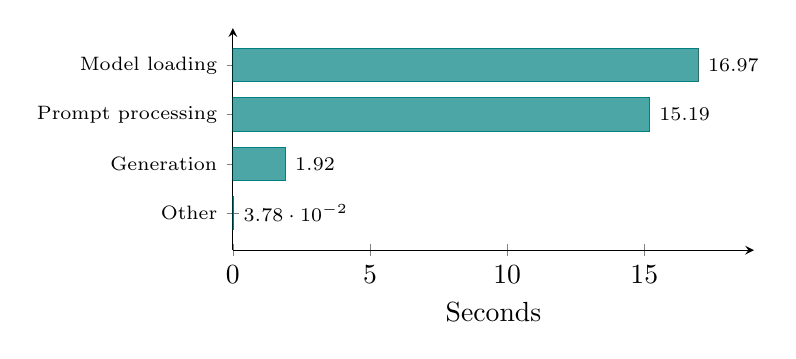
\begin{tikzpicture}\begin{axis}[width=8.2cm,height=4.4cm,xbar,xmin=0,xmax=19,ytick={1,2,3,4},yticklabels={Other,Generation,Prompt processing,Model loading},xlabel={Seconds},nodes near coords,nodes near coords align={horizontal},every node near coord/.append style={font=\scriptsize},bar width=12pt,axis lines=left,xtick={0,5,10,15},enlarge y limits=.25,yticklabel style={font=\scriptsize}]
\addplot[fill=teal!70,draw=teal] coordinates {(.0378,1)(1.916,2)(15.192,3)(16.967,4)};
\end{axis}\end{tikzpicture}
\column{.35\textwidth}\textbf{Actual local Llama call}\par
Client elapsed time: \textbf{34.113 s}.\par\medskip
1,891 prompt tokens; 137 generated tokens.\par\medskip
Most time came before token generation. A warm repeat can behave differently.\par\medskip
\textbf{Do not call a replay ``inference latency''.}
\end{columns}\Source{\href{https://docs.ollama.com/api/chat}{Ollama chat API: timing fields}; \href{../Classroom_Labs.html}{Executed tutorial: Classroom\_Labs, L0--L12}}
\Bridge{Place the assistant beside the control-room tools}
\note{This is the saved actual Llama 3.1 8B call from the optional classroom validation, not a new call made by the slide. Ollama reports its loading, prompt-processing and generation durations; the client timer includes the complete request. Small differences include server and transport overhead, so do not force the components to equal the client total exactly. The response chose RELAX\_Q\_10\_PERCENT on the original test\_01 context and requested a newly checked trial; it did not certify that future trial. Warm loading, prompt length and hardware can change latency substantially. Ask the audience whether this call belongs in a subsecond control loop or an advisory study. A deadline claim would require repeated end-to-end measurements, including failures and fallback. Transition: present this evidence in an operator-facing packet.}
\end{frame}

\begin{frame}[t]{How the workflow could fit beside control-room tools}\label{f:O01}
\centering\begin{tikzpicture}[x=1cm,y=1cm]
\node[box,text width=2.7cm] (d) at (-4.6,1.4) {Existing control-room data\\measurements + topology};
\node[box,text width=2.7cm] (s) at (0,1.4) {Advisory study workspace\\MPC, SAC, simulation, checks};
\node[box,text width=2.7cm] (o) at (4.6,1.4) {Operator workstation\\action, evidence, unresolved issues};
\draw[arrow] (d)--node[above,font=\scriptsize]{read}(s);\draw[arrow](s)--node[above,font=\scriptsize]{report}(o);
\node[box,text width=3.4cm,draw=slate,fill=white] (a) at (4.6,-1.4) {Existing authorized dispatch process\\outside this tutorial};
\draw[dashed,thick,slate](o)--node[right,font=\scriptsize]{separate authority}(a);
\node[text width=6.9cm,align=left] at (-2.5,-1.1) {The assistant assembles an engineering recommendation. A human reviews the evidence in the context of operating procedures.};
\end{tikzpicture}
\par\medskip The tutorial is an advisory sandbox with an explicit human boundary.
\Source{\href{https://arxiv.org/html/2609.22476v1}{Governance-aware TSO digital twin (2026)}; \href{../Classroom_Labs.html}{Executed tutorial: Classroom\_Labs, L0--L12}}
\Bridge{Which existing systems supply the study?}
\note{Follow the data path from the existing operational applications to a read-only study context, then through numerical candidates and verification to a reviewable recommendation. This is a deployment concept. The notebooks use a synthetic feeder and teaching cases; they do not connect to a live control system. The diagram should make the human review point prominent without suggesting that a dashboard alone establishes useful human oversight. An operator needs the relevant evidence at the right time and must be able to reject or request clarification. Ask which information belongs in a structured field rather than generated prose: equipment identifiers, limits, model scope and candidate identity are strong examples. Transition: trace the operational inputs, then rehearse each case before inspecting the review packet.}
\end{frame}

\newcommand{\OperatorIdea}[2]{\par\smallskip\begin{beamercolorbox}[sep=4pt,wd=\linewidth]{block body}{\fontsize{9}{10.5}\selectfont\color{teal}\bfseries #1\par}\smallskip{\fontsize{9}{10.5}\selectfont #2\par}\end{beamercolorbox}\smallskip}
\begin{frame}[t]{The study starts with a consistent operating snapshot}\label{f:D01}
\hyphenpenalty=10000\exhyphenpenalty=10000
\fontsize{9}{10.5}\selectfont\raggedright
\centering
\begin{tikzpicture}[x=1cm,y=1cm,scale=.84,transform shape]
\node[box,text width=3.1cm] (a) at (-4.8,2.1) {SCADA / ADMS\\measurements, switch status};
\node[box,text width=3.1cm] (b) at (-4.8,.55) {GIS / OMS\\assets and outages};
\node[box,text width=3.1cm] (c) at (-4.8,-1) {DERMS / forecasts\\available DER, expected load};
\uncover<2->{\node[box,text width=3.2cm] (s) at (0,.55) {Validated study snapshot\\time + quality flags\\revision + units};
\draw[arrow](a.east)--++(.4,0)|-(s.north west);\draw[arrow](b)--(s);\draw[arrow](c.east)--++(.4,0)|-(s.south west);}
\uncover<3->{\node[box,text width=3.1cm] (r) at (4.8,.55) {Awareness agent\\bind operator request\\to this snapshot};\draw[arrow](s)--(r);}
\end{tikzpicture}
\par\smallskip\fontsize{8}{9.2}\selectfont SCADA: supervisory control and data acquisition; ADMS: advanced distribution management system.\\
GIS: geographic information system; OMS: outage management system; DERMS: distributed energy resource management system.
\Question{What if the switch status and model describe different network revisions?}
\Answer{Hold the study and reconcile the snapshot before calculating a recommendation.}
\Source{Proposed integration, not implemented live. \href{https://www.nlr.gov/grid/adms-test-bed}{NLR ADMS Test Bed}; tutorial L1 and L7 demonstrate input/evidence binding.}
\Bridge{How do the notebook functions become services?}
\note{Begin with the systems an operator already uses. SCADA and an ADMS provide operational measurements and equipment status. A geographic information system supplies asset and connectivity information, while an outage management system supplies outage context. A DER management system can provide controllable resource availability. The diagram is a proposed interface pattern, not a claim that these systems are connected to the tutorial. Each utility has its own system boundaries and authoritative records. The first engineering task is to reconcile identifiers, units, timestamps, quality flags and topology into one study snapshot. A language model cannot resolve contradictory physical status by choosing a plausible sentence. L1 and L7 illustrate the narrower input-binding mechanism. For a live deployment, authentication, source integrity, clock handling and model maintenance are additional work. Ask the audience which system is authoritative for switch status in their organization.}
\end{frame}

\begin{frame}[t]{The assistant runs beside the existing control system}\label{f:D02}
\hyphenpenalty=10000\exhyphenpenalty=10000
\fontsize{9}{10.5}\selectfont\raggedright
\centering
\begin{tikzpicture}[x=1cm,y=1cm,scale=.94,transform shape]
\node[box,text width=2.8cm] (input) at (-4.9,1.8) {Read-only data adapter\\validated snapshot};
\node[box,text width=3.1cm] (flow) at (0,1.8) {Workflow service\\typed state, bounded routing};
\node[box,text width=2.8cm] (ui) at (4.9,1.8) {Operator display\\recommendation + evidence};
\draw[arrow](input)--(flow);\draw[arrow](flow)--(ui);
\uncover<2->{\node[box,text width=2.8cm] (llm) at (-4.9,-.3) {Local Ollama / Llama\\allowed response schema};
\node[box,text width=3.1cm] (tools) at (0,-.3) {Numerical workers\\MPC, SAC, MILP, WLS/QP\\LinDistFlow / OpenDSS};
\node[box,text width=2.8cm] (store) at (4.9,-.3) {Durable evidence store\\inputs, versions, results};
\draw[arrow](flow.south west)--(llm.north east);\draw[arrow](flow)--(tools);\draw[arrow](flow.south east)--(store.north west);}
\uncover<3->{\node[draw=red,fill=red!4,align=center,text width=12.8cm,inner sep=5pt,font=\small] at (0,-1.95) {Proposed service boundary: tool allowlist, deadlines and worker isolation.\\The LLM service receives no field-command credentials.};}
\end{tikzpicture}
\Source{Proposed architecture. \href{https://nvlpubs.nist.gov/nistpubs/SpecialPublications/NIST.SP.800-82r3.pdf}{NIST SP 800-82r3, \S5.2.3.1}; \href{https://docs.langchain.com/oss/python/langgraph/persistence}{LangGraph persistence}; tutorial G0--G5 and L0--L12.}
\Bridge{What appears on screen during a voltage alert?}
\note{Map each box back to something the audience has already run. The numerical functions become bounded jobs that accept typed inputs and return results, scope and timing. The workflow service coordinates these jobs. A local Llama service interprets requests or proposes allowed refinements, with responses validated against the allowed schema. Running Ollama locally does not by itself create an operational security boundary. A deployment needs controlled network paths, identities, restricted tool permissions and a durable evidence store. The graph lab's in-memory checkpoint is useful for teaching but does not survive a process restart; persistence and recovery must be engineered and tested. The tutorial's engineering supervisor and its separate LangGraph lab are also distinct implementations. Integrating them into this service architecture is proposed development. There is no implemented ADMS connector or equipment command gateway in this tutorial.}
\end{frame}

\begin{frame}[t]{Voltage desk: an alarm becomes a request for a checked action}\label{f:D03}
\hyphenpenalty=10000\exhyphenpenalty=10000
\fontsize{9}{10.5}\selectfont\raggedright
\begin{columns}[T,onlytextwidth]
\column{.47\textwidth}
\small\textbf{Illustrative operator request}\par
``High PV is raising voltage. Study a feasible inverter setting for the full feeder.''\par\smallskip
\begin{tikzpicture}[x=1cm,y=.78cm]
\node[box,text width=6.2cm,font=\small] (a) at (0,0) {Awareness: snapshot + full scope};
\uncover<2->{\node[box,text width=6.2cm,font=\small] (p) at (0,-1) {Planning: MPC / saved SAC candidates};\draw[arrow](a)--(p);
\node[box,text width=6.2cm,font=\small] (s) at (0,-2) {Simulation: LinDistFlow / OpenDSS};\draw[arrow](p)--(s);
\node[box,text width=6.2cm,font=\small] (v) at (0,-3) {Verification: voltage / current / scope};\draw[arrow](s)--(v);
\node[box,text width=6.2cm,font=\small] (r) at (0,-4) {LLM Optimizer: refine and recheck};\draw[arrow](v)--(r);}
\end{tikzpicture}
\column{.49\textwidth}
\uncover<3->{\OperatorIdea{Evidence from the tutorial}{Same-action audit across 12 test cases:\par MV check: 12/12 pass.\par Full MV/LV AC check: 0/12 pass.\par\smallskip\textcolor{red}{MV evidence cannot certify the full-feeder request.}}
\textbf{Operator display}\par
Status: HOLD for broader evidence.\par
Next study: repair and validate at full scope.\par
Examples: L5/L12; batch: paired-model pilot.}
\Question{What would a useful assistant save the operator from doing manually?}
\uncover<4->{\Answer{Assembling model scope and conflicting checks into one reviewable record.}}
\end{columns}
\Source{Illustrative scenario. 12-case audit: \href{../LLM_Response_Selection.html}{recorded paired-model pilot}. One-case demo: L5; scope packet: L12. No field dispatch occurred.}
\Bridge{How does the operator's service priority change restoration?}
\note{This screen is a teaching storyboard, not a screenshot of a deployed utility product. Start with the operator's request and underline full feeder. The model scope is part of the request, not a footnote added after solving. MPC and the saved SAC policy generate alternatives, and simulations evaluate their electrical consequences. The twelve-case result comes from the recorded model audit and must not be described as twelve events on a live network. Its value here is to show why a narrow green check can be misleading. The framework can organize the evidence, propose a permitted next study and make the missing scope visible. It has not demonstrated a reduction in operator workload; that requires a human comparison. A fixed supervisory application with the same scope check can also hold this request. The potential language benefit is interpreting varied requests and explaining tool evidence accurately.}
\end{frame}

\begin{frame}[t]{Restoration desk: the service priority is visible before review}\label{f:D04}
\hyphenpenalty=10000\exhyphenpenalty=10000
\fontsize{9}{10.5}\selectfont\raggedright
\begin{columns}[T,onlytextwidth]
\column{.48\textwidth}
\small\textbf{Illustrative operator request}\par
``The fault is isolated. Compare pickup plans that prioritize the two critical loads.''\par\smallskip
\begin{tikzpicture}[scale=.68,transform shape]
\RestMap{40}
\end{tikzpicture}
\par\smallskip\footnotesize Six-node fixture; isolation is assumed in this story.
\column{.49\textwidth}
\uncover<2->{\small\begin{tabularx}{\linewidth}{Xrr}\toprule Plan & Total kW & Critical kW\\\midrule
Unweighted & 140 & 30\\Weighted & 130 & 90\\\bottomrule\end{tabularx}
\OperatorIdea{Proposed operator display}{Requested policy: critical-load weights.\par Candidate: weighted MILP solution.\par Next: engineering and switching review.}}
\uncover<3->{\small Awareness: status. Planning: MILP. Simulation: candidate network. Verification: limits and evidence. LLM Optimizer: request a permitted refinement.}
\end{columns}
\Question{Does the higher critical service prove an LLM advantage?}
\Answer{No. It follows from the objective. A fixed workflow with the same MILP can achieve it.}
\Source{Recorded Classroom\_Labs L6--L7. Active-power transport model, not an AC switching certification. \href{https://www.nlr.gov/grid/adms-test-bed}{NLR ADMS Test Bed} illustrates a route to lab integration.}
\Bridge{Where does Llama help interpret the operator's words?}
\note{Ask a learner to point to the failed segment and the two ties before discussing the table. This reconnects the control-room request to the physical topology taught earlier. The statement that the fault is isolated is an assumption in this illustrative story; the notebook does not validate work permits, field isolation or protection coordination. Both numerical rows are real outputs from the classroom fixture. Their difference reflects different service objectives. The assistant's proposed contribution is to interpret and confirm the requested priority, call the appropriate study, preserve the chosen objective and summarize the tradeoff. It does not create the mathematical gain. The operator still needs the operational switching procedure and the utility's engineering checks. Explain that the classroom transport calculation is a limited simulation; a utility pilot would add suitable AC, protection and temporal switching studies before treating the recommendation as operationally actionable.}
\end{frame}

\begin{frame}[t]{A useful Llama role: understand the operator's restriction}\label{f:D04B}
\hyphenpenalty=10000\exhyphenpenalty=10000
\centering
\begin{tikzpicture}[x=1cm,y=1cm]
\node[box,text width=5.95cm,align=left,anchor=north,font=\footnotesize] (request) at (-3.9,2.8) {\textbf{Saved operator request h06}\\[4pt]
``Use the 0.25 km bypass to reconnect demand, with current no higher than \textbf{100 A}. Keep the 2 km bypass \textbf{open} and leave PV generation at \textbf{zero}.''\par\smallskip
\scriptsize The request restricts a permitted study; it cannot remove fault quarantine.};
\uncover<2->{
\node[box,text width=6.1cm,align=left,anchor=north,font=\footnotesize] (fields) at (3.85,2.8) {\textbf{Actual saved Llama fields}\\[3pt]
{\ttfamily\fontsize{7.2}{8.5}\selectfont\renewcommand{\arraystretch}{.8}
\begin{tabular}{@{}l@{}}
\{\\
\quad "status": "READY",\\
\quad "rating\_fraction": 1.0,\\
\quad "short\_limit\_amps": 100,\\
\quad "allow\_long\_tie": false,\\
\quad "allow\_pv": false,\\
\quad "reason": "Operator request accepted as is"\\
\}
\end{tabular}}\par};
\draw[arrow] (request.east)--node[above,font=\scriptsize]{interpret}(fields.west);
}
\end{tikzpicture}\par
\uncover<2->{\footnotesize \texttt{READY} is an interpretation status; numerical feasibility still requires a separate check.}\par\smallskip
\uncover<3->{
\footnotesize\renewcommand{\arraystretch}{1}
\begin{tabularx}{.95\linewidth}{Xcc}\toprule
Seven authored requests (post-hoc subset) & Documented parser & Parser + Llama\\\midrule
Clear requests completed correctly & 3/5 & 5/5\\
Missing/prohibited requests clarified & 2/2 & 2/2\\
Actual Llama calls across this subset & 0 & 4\\\bottomrule
\end{tabularx}\par\smallskip
\raggedright\footnotesize
\textbf{Saved h06 call: 3.160 s.} Historical feeder catalog + OpenDSS, separate from L6's six-node MILP.\\
The observed gain is request interpretation against this parser; better optimization and operator-time savings were not established.
}
\Source{\href{../results/confirmation_calls.json}{Actual saved h06 request, schema, response and client duration}; \href{../results/case_comparison_evidence.json}{Recorded restoration comparison: five clear and two clarification cases}.}
\Bridge{When measurements are suspect, what evidence can the operator trust?}
\note{Begin with the operator's request and ask the audience to identify its three restrictions before revealing the response. The short bypass has a 100 ampere ceiling, the long bypass is unavailable by instruction, and PV must remain zero. Llama returns those restrictions in a fixed schema; rating\_fraction stays at the trusted default of one. READY describes interpretation only. The recorded h06 call took 3.160 seconds of client elapsed time. Across this descriptive subset, the documented parser completed three of five clear requests, while parser followed by Llama completed all five. Both clarified both missing or prohibited requests. Four Llama calls were used in total. These historical feeder catalog experiments are separate from L6's six-node MILP. The evidence supports request interpretation against this parser, not improved optimization or measured operator workload. Next, contrast a clear operator request with measurements whose trust is uncertain.}
\end{frame}

\begin{frame}[t]{Cyber desk: a quiet residual still needs a trustworthy basis}\label{f:D05}
\hyphenpenalty=10000\exhyphenpenalty=10000
\fontsize{9}{10.5}\selectfont\raggedright
\begin{columns}[T,onlytextwidth]
\column{.48\textwidth}
\small\textbf{Illustrative operator request}\par
``A power-flow estimate looks plausible, but measurements may be corrupted. What evidence supports a correction?''\par\medskip
\begin{tikzpicture}[x=1cm,y=1cm,scale=.94,transform shape]
\node[box,text width=5.7cm] (m) at (0,1.4) {Awareness + WLS\\Residual $J\approx3.9202$};
\uncover<2->{\node[box,text width=2.2cm,draw=red] (h) at (-1.65,-.6) {No justified trusted data\\HOLD / escalate};
\node[box,text width=2.2cm] (q) at (1.65,-.6) {Trusted-data assumption\\QP candidate};
\draw[arrow](m)--node[left,font=\scriptsize]{absent}(h);\draw[arrow](m)--node[right,font=\scriptsize]{available}(q);}
\end{tikzpicture}
\column{.49\textwidth}
\uncover<3->{\OperatorIdea{Recorded four-bus result}{QP injection: $u\approx0.12169$ p.u.\par Simulated true branch flow:\par $0.17046\leq0.18$ p.u.\par Fixed and Llama supervisors return the same final $u$.}
\small Planning requests the constrained correction. Simulation predicts its consequence. Verification checks flow and the declared data assumption. The LLM Optimizer can retain or refine only within those conditions.}
\end{columns}
\Question{Can an LLM explanation establish that a sensor is trustworthy?}
\uncover<4->{\Answer{No. Provenance and independent operational evidence must support that assumption.}}
\Source{Recorded Classroom\_Labs L8--L9 and archived trace. \href{https://doi.org/10.1145/1653662.1653666}{Liu, Ning \& Reiter, CCS 2009}; protected angles are assumed trusted in this teaching model.}
\Bridge{What separates a recommendation from an executed change?}
\note{The residual value illustrates the coordinated corruption case, where the measurements can remain internally consistent while the inferred state is wrong. It is a recorded synthetic result, not an attack detector for a live utility. The trusted-data branch uses protected angle measurements that the teaching code assumes are available and trustworthy. A deployed system must establish that basis through operational security and measurement provenance; an LLM cannot supply it by assertion. The constrained quadratic program produces the reported action, and the synthetic true flow is available for offline evaluation. A control room would not have unrestricted access to hidden ground truth. The fixed and language-assisted supervisors return the same correction in this trace. The potential workflow value is explicit escalation, tool coordination and explanation, while the correction itself comes from the numerical method.}
\end{frame}

\begin{frame}[t]{Operator acknowledgment and field execution are different events}\label{f:D06}
\hyphenpenalty=10000\exhyphenpenalty=10000
\fontsize{9}{10.5}\selectfont\raggedright
\centering\begin{tikzpicture}[x=1cm,y=1cm,scale=.94,transform shape]
\node[box,text width=2.6cm] (p) at (-4.9,1.6) {Checked proposal\\candidate ID + revision};
\node[box,text width=2.6cm] (r) at (0,1.6) {Operator review\\acknowledge / reject / study};
\node[box,text width=2.6cm,draw=slate,fill=white] (d) at (4.9,1.6) {Existing authorized process\\dispatch decision};
\draw[arrow](p)--(r);\draw[dashed,arrow](r)--node[above,font=\scriptsize]{separate authority}(d);
\uncover<2->{\node[box,text width=2.6cm,draw=slate,fill=white] (x) at (4.9,-1) {Field response\\status + measurements};
\node[box,text width=2.6cm,draw=slate,fill=white] (c) at (0,-1) {Post-action check\\expected versus observed};
\draw[dashed,arrow](d)--(x);\draw[dashed,arrow](x)--(c);}
\node[align=left,text width=3.4cm,font=\small] at (-4.8,-.85) {Solid path: tutorial advisory record.\\Dashed path: proposed integration, absent from the notebook.};
\end{tikzpicture}
\Question{If the device does not reach the expected state, should the assistant mark the job complete?}
\Answer{No. Preserve the discrepancy and hand it to the established operating procedure.}
\Source{Proposed integration and tutorial L12 boundary. \href{https://airc.nist.gov/airmf-resources/airmf/5-sec-core/}{NIST AI RMF: GOVERN 3.2, MANAGE 2.4 and 4.1}.}
\Bridge{How should delayed or unavailable advice be handled?}
\note{Use the two rows to distinguish two kinds of readback. In the tutorial, the human acknowledgment names a checked candidate. In an operational deployment, field readback means observing equipment state and measurements after an authorized command. These are separate events and need separate records. The notebook implements only advisory acknowledgment, and its equipment-dispatch flag remains false. A future command gateway would require independent authorization, equipment interlocks and the utility's operating procedure. The proposed post-action check compares expected and observed consequences and preserves discrepancies instead of automatically declaring success. It must not issue an improvised rollback, because the safe response depends on the current physical state. Ask participants to name the system and role responsible for dispatch in their own control room. The assistant supports that responsibility rather than assuming it.}
\end{frame}

\begin{frame}[t]{Slow advice must not delay the existing control response}\label{f:D07}
\hyphenpenalty=10000\exhyphenpenalty=10000
\fontsize{9}{10.5}\selectfont\raggedright
\begin{columns}[T,onlytextwidth]
\column{.53\textwidth}
\begin{tikzpicture}[x=1cm,y=1cm,scale=.94,transform shape]
\node[box,text width=6.5cm] (s) at (0,1.9) {Study starts at $t_0$\\snapshot revision $r$, candidate $u$};
\uncover<2->{\node[box,text width=6.5cm] (g) at (0,.15) {Before review: still valid?\\$t_{\rm now}\leq t_{\rm valid}$ and revision unchanged};\draw[arrow](s)--(g);}
\uncover<3->{\node[box,text width=2.5cm] (a) at (-1.8,-1.6) {yes\\continue review};\node[box,text width=2.5cm,draw=red] (b) at (1.8,-1.6) {no / tool timeout\\expire study, notify};\draw[arrow](g)--(a);\draw[arrow](g)--(b);}
\end{tikzpicture}
\column{.43\textwidth}
\OperatorIdea{Measured example}{One local Llama call took 34.11 s, including 16.97 s loading. This is one measurement, not a service guarantee.}
\small $t_{\rm valid}$: site-defined evidence expiry.\par $r$: network/data revision.\par $u$: proposed control vector.\par\medskip
Design requirement: existing protection and approved controllers continue independently. A failed advisory service must not block them.
\end{columns}
\Source{Recorded L11 call; \href{https://docs.ollama.com/api/chat}{Ollama timing fields}. Proposed expiry/failure handling informed by \href{https://nvlpubs.nist.gov/nistpubs/SpecialPublications/NIST.SP.800-82r3.pdf}{NIST SP 800-82r3, OT performance and availability}.}
\Bridge{What would a credible deployment pilot look like?}
\note{The observed Llama duration is useful because it prevents treating a language-model call as an instantaneous part of a protective control loop. It is a single recorded call, including model loading, so it does not establish a latency distribution or an operational service-level target. A pilot should measure warm and cold calls, queueing, tool execution and total recommendation time. The proposed validity check makes freshness explicit. Its deadline must come from the use case and the utility's operating requirements, not from an arbitrary number on a slide. A changed topology or expired snapshot can invalidate an otherwise well-formed result. The teaching notebook demonstrates revision binding but does not implement a production deadline scheduler. On advisory failure, established protection and approved control procedures continue; the assistant reports the incomplete study without inventing a replacement control action.}
\end{frame}

\begin{frame}[t]{A deployment pilot earns authority through measured evidence}\label{f:D08}
\hyphenpenalty=10000\exhyphenpenalty=10000
\fontsize{9}{10.5}\selectfont\raggedright
\centering\begin{tikzpicture}[x=1cm,y=1cm,scale=.94,transform shape]
\node[box,text width=2.65cm] (a) at (-5,1.7) {1. Offline replay\\historical / synthetic cases};
\node[box,text width=2.65cm] (b) at (-1.67,1.7) {2. Laboratory tests\\ADMS / device interfaces};
\node[box,text width=2.65cm] (c) at (1.67,1.7) {3. Read-only shadow\\compare with actual decisions};
\node[box,text width=2.65cm] (d) at (5,1.7) {4. Supervised advisory\\operators can reject};
\draw[arrow](a)--(b);\draw[arrow](b)--(c);\draw[arrow](c)--(d);
\uncover<2->{\node[draw=teal,fill=pale,text width=12.7cm,align=left,inner sep=7pt,font=\small] at (0,-.2) {\textbf{Compare against the same approved fixed workflow}\par
Correct studies selected; constraint violations missed; stale evidence accepted; operator decision time; rejected recommendations; median and 95th-percentile total latency.};}
\uncover<3->{\node[align=center,text width=12.5cm,font=\small] at (0,-1.75) {Define acceptance criteria before the pilot. Include outages, bad data and unavailable tools.\\Retain the fixed workflow when the assistant adds no measured benefit.};}
\end{tikzpicture}
\Source{Proposed staged pilot, not a mandated sequence. \href{https://www.nlr.gov/grid/adms-test-bed}{NLR ADMS Test Bed}; \href{https://airc.nist.gov/airmf-resources/airmf/5-sec-core/}{NIST AI RMF MEASURE 2.3}; \href{https://www.energy.gov/oe/grid-control-and-data-science}{DOE Grid Control and Data Science}.}
\Bridge{Which parts can we rehearse with the current notebook?}
\note{Describe this as a proposed evaluation path. The cited laboratory demonstrates that realistic ADMS and DERMS integration can be tested with simulated networks and hardware interfaces; it does not validate our agentic workflow. Offline replay first checks reproducibility and failure behavior. Laboratory integration then exposes interface and timing issues. Read-only shadow operation consumes approved data and records recommendations while the established workflow remains authoritative. A supervised advisory pilot adds operator interaction after acceptance criteria are met. There is no automatic graduation to autonomous control on this slide. For scientific evaluation, match the cases, objectives, available information and computational budgets. Measure human decision quality and time with an appropriate study design before claiming workload savings. Report how often the baseline is better, and include failures and latency tails rather than only successful average cases.}
\end{frame}

\begin{frame}[t]{A four-minute rehearsal connects the desk to the notebook}\label{f:D09}
\hyphenpenalty=10000\exhyphenpenalty=10000
\fontsize{9}{10.5}\selectfont\raggedright
\small\begin{tabularx}{\linewidth}{p{2.15cm}XX}\toprule Control-room event & Notebook evidence & Operator's explanation\\\midrule
Voltage alert & L5 model audit; L12 scope mismatch & Why does an MV pass leave a full-feeder request on HOLD?\\
Restoration request & L6 service tradeoff; L7 changed rating & Which objective was requested, and does the old evidence still apply?\\
Suspect telemetry & L8 residual; L9 trusted-data QP & What supports the measurement assumption before any corrective recommendation?\\\bottomrule\end{tabularx}
\uncover<2->{\OperatorIdea{Work in pairs}{One person acts as operator, the other as the assistant. Choose one row, inspect the saved output, and state: decision, missing evidence, next tool or responsible person.}}
\uncover<3->{\small\textbf{Instructor check:} A clear response cites the numerical result and its scope. It can legitimately end with a hold or a request for another study.}
\Source{Tutorial Classroom\_Labs L5--L9 and L12. Rehearsal is educational; the saved outputs do not certify a real operating decision.}
\Bridge{Now inspect the exact packet that can be acknowledged.}
\note{Allow four minutes within the operator segment. This activity uses already computed outputs rather than requiring a new model installation or a long Llama call. Assign one event to each pair so they have time to inspect evidence instead of skimming all three cases. The person playing the assistant should point to a field or number, identify its model scope and explain the next step. The operator should ask one challenge question, such as whether the topology changed, whether the full feeder was checked or why the trusted measurement assumption is justified. Swap roles if time permits. This rehearsal is a teaching activity, not a measured usability experiment. Its purpose is to connect the mathematical and software lessons to a recognizable control-room exchange. The next slides run the exact L12 acknowledgment checks.}
\end{frame}

\begin{frame}[t]{The operator sees scope before readback}\label{f:O02}
\small\textbf{Saved recommendation ID:} \texttt{b67cff9c8eb444c2}\par\medskip
\begin{tabularx}{\linewidth}{lXX}\toprule Packet field & Full MV/LV request & Explicit MV teaching request\\\midrule
Verified scope & MV phases only & MV phases only\\
Scope matches & No & Yes\\
State & HOLD & READY\_FOR\_READBACK\\
Acknowledged & False & True\\
Equipment dispatch & False & False\\
\bottomrule\end{tabularx}\Question{The numerical evidence is the same. Why is only the second packet eligible?}\Answer{The second request asks only for the scope that was checked. The first asks for more. Acknowledgment still does not dispatch equipment.}
\Source{\href{../Classroom_Labs.html}{Executed tutorial: Classroom\_Labs, L0--L12}; \href{https://arxiv.org/html/2609.22476v1}{Governance-aware TSO digital twin (2026)}}
\Bridge{Acknowledgment is a guarded transition}
\note{Present the action and its identity first, then the supporting evidence. A reviewer should not have to reconstruct the proposal from a long chat transcript. Include the requested and verified model scope, the age of the evidence, numerical constraint margins, rejected alternatives and a concise public rationale tied to tool results. In this tutorial the most consequential scope distinction is the MV-only result versus the broader MV/LV requirement. A polished summary cannot silently expand that scope. Invite learners to remove one field and predict the resulting ambiguity. Removing the identifier obscures which candidate was reviewed; removing the scope can turn a valid limited statement into an unsupported general claim. Transition: acknowledgment changes a specific state, not the physical network.}
\end{frame}

\begin{frame}[t]{Acknowledgment is a guarded transition}\label{f:O03}
\begin{columns}[T]\column{.47\textwidth}\centering\begin{tikzpicture}[x=1cm,y=1cm]
\node[box,text width=2.7cm] (a) at (0,2.4) {Candidate is checked};
\node[box,text width=2.7cm] (b) at (0,.9) {Required scope matches};
\node[box,text width=2.7cm] (c) at (0,-.6) {Matching readback recorded};
\draw[arrow](a)--(b);\draw[arrow](b)--(c);
\node[align=center,font=\small,text=red] at (0,-1.7) {Advisory acknowledgment\\equipment dispatch remains false};
\end{tikzpicture}\column{.50\textwidth}
\textbf{Only a matching, eligible packet can be acknowledged.}\par\medskip
\begin{itemize}\item Proposed \ensuremath{\rightarrow} checked\item Checked \ensuremath{\rightarrow} awaiting review\item Matching readback \ensuremath{\rightarrow} acknowledged\end{itemize}
\end{columns}
\Source{\href{../Classroom_Labs.html}{Executed tutorial: Classroom\_Labs, L0--L12}; \href{../Graph_Workflow_Lab.html}{Executed LangGraph teaching lab: G0--G5}; \href{https://docs.langchain.com/oss/python/langgraph/interrupts}{LangGraph: interrupts and resume}}
\Bridge{Code: bind review to the candidate}
\note{Animate the review path one state at a time. The conceptual sequence distinguishes calculation, review readiness and human acknowledgment. In the implementation, a full MV/LV request supported only by an MV result is held; an explicitly limited MV teaching request can become eligible for acknowledgment. The candidate identifier binds the readback to a particular packet. Emphasize that these are advisory application states. They neither authenticate a real operator nor dispatch equipment. The earlier LangGraph G5 exercise demonstrated interruption and resumption using a checkpoint, while L12 demonstrates the engineering packet checks. They teach related ideas through separate code paths. Ask the audience to identify which failure should stop the path before any readback is accepted. Transition: inspect the exact L12 statements.}
\end{frame}

\begin{frame}[t]{Code: bind review to the candidate}\label{f:O04}
\Checkpoint{L12}{Exact notebook excerpt; run the complete cell in order.}
\Code{O04.py}
\Idea{What the code means}{A wrong candidate ID cannot acknowledge the packet.}
\begin{itemize}\item First request uses a wrong ID\item Second reads back the packet ID\item The operator label is a classroom placeholder\end{itemize}
\Source{\href{../Classroom_Labs.html}{Executed tutorial: Classroom\_Labs, L0--L12}}
\Bridge{Hands-on: read back, reject, inspect}
\note{Read these two notebook lines aloud. The first call deliberately supplies the wrong recommendation identifier. The second uses the identifier carried by the eligible MV teaching packet. Both calls go to ordinary Python logic, so the readback rule is inspectable independently of language-model output. The string Student operator is an instructional placeholder rather than an authentication mechanism. Keep the previously constructed packet visible: it records what was checked and under which scope. This exact excerpt comes from L12 of Classroom\_Labs, and learners should run L0--L5 first so the selected-trial context exists. Ask them to predict the two outcomes before running the cell. Transition: run the full packet exercise, then inspect its assertions.}
\end{frame}

\begin{frame}[t]{Hands-on: read back, reject, inspect}\label{f:O05}
\Idea{Four-minute notebook exercise}{Use L12 to distinguish scope, identity and acknowledgment.}
\begin{enumerate}\item Run L12 after its earlier cells\item Find the full-scope HOLD\item Inspect the wrong-ID rejection\item Confirm no equipment dispatch\end{enumerate}
\Question{Which of the three outcomes is permission to dispatch equipment?}
\Answer{None. Even the acknowledged packet is explicitly advisory.}
\Source{\href{../Classroom_Labs.html}{Executed tutorial: Classroom\_Labs, L0--L12}}
\Bridge{The checks distinguish three outcomes}
\note{Give learners four minutes and keep this slide visible. First run the unmodified L12 cell after the earlier classroom cells. Inspect the displayed packet for the full MV/LV requirement and compare it with the explicitly MV teaching packet. Then inspect wrong\_id in a scratch cell; it is intentionally not the accepted readback. Finally check the three assertions at the end of L12. Have partners explain the difference between an eligible packet and an acknowledged packet. Avoid changing the original assertion expectations during the first run. For an extension, discuss which fields would change if the requested control changed and which evidence would need to be recomputed. This is a local advisory exercise; the notebook has no equipment-dispatch endpoint. Transition: compare the predicted outcomes with the executed checks.}
\end{frame}

\begin{frame}[t]{The checks distinguish three outcomes}\label{f:O06}
\Checkpoint{L12}{Exact notebook excerpt; run the complete cell in order.}
\Code{O06.py}
\Idea{What the code means}{Scope mismatch holds; wrong identity rejects; valid readback remains advisory.}
\begin{itemize}\item Full MV/LV requirement: HOLD\item Wrong identifier: REJECTED\item Matching MV readback: acknowledged\end{itemize}
\Source{\href{../Classroom_Labs.html}{Executed tutorial: Classroom\_Labs, L0--L12}}
\Bridge{A changed request needs new evidence}
\note{Show the assertions after learners have made their predictions. They are deliberately more precise than an all-purpose PASS label. The full-scope packet is held because the supporting model is narrower than the request. The wrong identifier is rejected because it does not name the current packet. The eligible MV packet can be acknowledged, yet its equipment-dispatch flag remains false. These outcomes demonstrate the logic of the teaching application, not authentication, field authorization or human comprehension. Ask a participant to explain why the first failure cannot be repaired by entering the right identifier. It requires suitable evidence for the requested scope or an explicitly changed request, followed by the corresponding review. Transition: examine what happens when the underlying request changes.}
\end{frame}

\begin{frame}[t]{A smaller current limit changes the decision}\label{f:O07}
\begin{columns}[T]\column{.47\textwidth}\centering\begin{tikzpicture}[x=1cm,y=1cm]
\node[box,text width=3.7cm] (a) at (0,2.2) {Old record\\$u=0.50$, limit $=0.80$, revision 1};
\node[box,text width=3.7cm,draw=red] (b) at (0,.4) {Changed request\\same action, limit $=0.70$, revision 2};
\draw[arrow](a)--node[right,font=\scriptsize]{old check cannot transfer}(b);
\node[box,text width=3.7cm] at (0,-1.4) {Recalculate: $i=0.4+0.8(0.5)=0.8$\\$0.8>0.7$: HOLD};
\end{tikzpicture}\column{.50\textwidth}
\textbf{A hash links content; it does not establish physical truth.}\par\medskip
$u$ is the proposed control; $i$ is the toy current. This uses the opening scalar model, not a feeder calculation.\par\medskip
\begin{itemize}\item Change a limit or candidate\item Old binding no longer matches\item Recompute the affected study\end{itemize}
\Question{Can the old acknowledgment survive a changed control?}
\end{columns}
\Source{\href{../Classroom_Labs.html}{Executed tutorial: Classroom\_Labs, L0--L12}}
\Bridge{Capstone: approve review, hold or request a study?}
\note{Connect this question to L1 and L7, where the classroom explicitly checks stale bindings after a request or candidate changes. The binding helps detect a mismatch between saved evidence and its stated inputs. It does not prove that a sensor is trustworthy, that a model is correct or that an operator is authorized. Ask learners to identify the smallest changed field that should invalidate the old check: a current limit, load scale, topology revision or control setting all provide concrete examples. Their answer should include the affected numerical step, not only a request for a new language explanation. The important habit is to preserve evidence provenance through revision. Transition: apply this habit to three operator decision cards.}
\end{frame}

\begin{frame}[t]{Capstone: approve review, hold or request a study?}\label{f:O08}
\Idea{Work with a partner}{Name the missing evidence and the next responsible step.}
\begin{enumerate}\item A: MV PASS; full-feeder AC FAIL\item B: restoration PASS; isolation record absent\item C: no alarm; protected measurements absent\end{enumerate}
\Question{For your card, identify one missing fact and the next tool or human step.}
\Answer{A: broader-model repair. B: authorized isolation evidence. C: justified independent measurements or escalation.}
\Source{\href{../Classroom_Labs.html}{Executed tutorial: Classroom\_Labs, L0--L12}; \href{https://doi.org/10.1145/1653662.1653666}{Liu, Ning \& Reiter, false-data injection, CCS 2009}}
\Bridge{Five stages, three cases, one evidence discipline}
\note{Give each group one card and ask for a decision plus a concrete next step. Card A requires repair or another study at the requested model scope; a confident Llama sentence cannot override the AC failure. Card B exposes a missing operational prerequisite: a feasible mathematical switching plan is not proof of authorized isolation. Card C exposes incomplete information: an unalarmed residual alone cannot establish trustworthy state estimation under the constructed stealth attack. In each response, separate the numerical tool that can help from the authority or external evidence that the tool cannot invent. Do not assume that retaining an old setting is always safe after a changed topology or measurement regime. Use the final minute to compare the three different gaps. Transition: summarize how all five stages contribute.}
\end{frame}

\begin{frame}[t]{Five stages, three cases, one evidence discipline}\label{f:S01}
\small\begin{tabularx}{\linewidth}{lXXX}\toprule Stage & Voltage & Restoration & Cyber response\\\midrule
Awareness & Operating point and limits & Fault, ties, load priorities & Measurements and trust assumptions\\
Planning & MPC; SAC candidate & Weighted pickup MILP & Constrained recovery QP\\
Simulation & Network response & Flow on selected paths & Estimated / evaluated flows\\
Verification & Voltage/current and scope & Capacity, connectivity, binding & Residual and protected-data basis\\
LLM Optimizer & Propose a permitted refinement & Explain or request a revised trial & Explain or request additional evidence\\\bottomrule
\end{tabularx}\par\medskip
The numerical method changes with the decision. The record passed between stages keeps the action, assumptions and results together.
\Question{Which stage would catch a stale network revision?}\Answer{The evidence-binding check in Verification; a fluent summary cannot repair the mismatch.}\Source{\href{../Classroom_Labs.html}{Executed tutorial: Classroom\_Labs, L0--L12}; \href{../LLM_Response_Selection.html}{Recorded voltage pilot: E1--E8}}
\Bridge{Choose the simplest sufficient workflow}
\note{Invite one learner per use case to trace a single candidate through the five proposed stages. Awareness establishes measurements, constraints and model scope. Planning calls the relevant numerical formulation. Simulation computes the consequence of candidate controls; verification checks the declared requirements and binds the result. The optimizer can request a bounded refinement or retain an incumbent, after which the relevant evidence is checked again. Human review is the subsequent authority boundary, not a sixth language agent. For voltage this includes MPC and SAC candidate comparison; restoration uses a weighted service formulation; cyber response distinguishes estimation evidence from protected-information assumptions. The methods change while the handoff discipline remains. Transition: choose how much orchestration the task actually requires.}
\end{frame}

\begin{frame}[t]{Choose the simplest sufficient workflow}\label{f:S02}
\begin{columns}[T]\column{.47\textwidth}\centering\begin{tikzpicture}[x=1cm,y=1cm]
\node[box,text width=3.4cm] (a) at (0,2.1) {Are the next steps known in advance?};
\node[box,text width=1.8cm] (b) at (-1.5,.2) {Fixed controller + checks};
\node[box,text width=1.8cm] (c) at (1.5,.2) {Explicit routing / repair};
\draw[arrow](a)--node[left,font=\scriptsize]{yes}(b);\draw[arrow](a)--node[right,font=\scriptsize]{sometimes}(c);
\node[align=left,text width=4.6cm,font=\small] at (0,-1.5) {Add language interpretation only where requests or evidence require it. Test whether it improves a measured outcome.};
\end{tikzpicture}\column{.50\textwidth}
\textbf{Add an agent only when it addresses a measured task need.}\par\medskip
\begin{itemize}\item Repeated calculation \ensuremath{\rightarrow} fixed workflow\item Varied requests \ensuremath{\rightarrow} typed LLM interface\item Independent studies \ensuremath{\rightarrow} specialist coordination\end{itemize}
\end{columns}
\Source{\href{https://arxiv.org/abs/2512.08296v3}{Kim et al., scaling agent systems (2026)}; \href{../Graph_Workflow_Lab.html}{Executed LangGraph teaching lab: G0--G5}}
\Bridge{A reproducible result carries its context}
\note{Treat this as a design decision rather than a contest between labels. A stable calculation with known inputs can be well served by a fixed workflow. Language interpretation becomes useful when users express varied requests, but the resulting tool calls still need validation. Specialist coordination can help when responsibilities and evidence streams differ; it also adds communication overhead and potential handoff failures. Recent agent-scaling research motivates testing that tradeoff instead of assuming that a larger team is better. The classroom direct-Python and LangGraph comparison is deliberately equivalent on its toy cases: orchestration structure alone should not change the mathematics. Ask participants which part of their own workflow is currently variable or error-prone. Transition: preserve enough information to make that improvement measurable.}
\end{frame}

\begin{frame}[t]{A reproducible result carries its context}\label{f:S03}
\begin{columns}[T]\column{.47\textwidth}\centering\begin{tikzpicture}[x=1cm,y=1cm]
\node[draw=teal,fill=pale,rounded corners,align=left,font=\small,text width=5.4cm,inner sep=8pt] at (0,.6) {\textbf{Experiment record}\\[4pt]Scenario: load, topology, revision\\Candidate: control values + ID\\Model: equations + network scope\\Checks: margins and failed limits\\Time: solver, LLM, full workflow\\Decision: accept for review / HOLD};
\end{tikzpicture}\column{.50\textwidth}
\textbf{Archive the inputs, methods, outputs and evidence mode together.}\par\medskip
\begin{itemize}\item Case, model scope and data revision\item Solver, policy and LLM versions\item Seeds, budgets and measured durations\end{itemize}
\end{columns}
\Source{\href{../Classroom_Labs.html}{Executed tutorial: Classroom\_Labs, L0--L12}; \href{../LLM_Response_Selection.html}{Recorded voltage pilot: E1--E8}; \href{https://docs.ollama.com/api/chat}{Ollama chat API: timing fields}}
\Bridge{Design your next experiment}
\note{Use this checklist to prepare a reproducible scientific report, not a new permission process. The code cells already distinguish fresh numerical calculations, inference from saved SAC weights and archived actual LLM responses. The optional local Llama call is disabled by default, and its saved validation record includes a timestamp and timing fields. A screenshot of an answer is weaker than the structured record that identifies its request, model and tool results. Include failures and rejected alternatives where they affect interpretation. For the selector pilot, preserve the training, validation and held-out split and state that test-time learning was frozen. Ask learners to locate one such field in the supplied outputs. Transition: turn the remaining limitations into a clear next experiment.}
\end{frame}

\begin{frame}[t]{Design your next experiment}\label{f:S04}
\Idea{Work with a partner}{Change one factor and state what would falsify your claim.}
\begin{enumerate}\item Hypothesis: name the expected benefit\item Control: retain a strong fixed baseline\item Measure: outcome, failures and latency\item Boundary: state the model and task scope\end{enumerate}
\Question{Write one testable benefit and one result that would refute it.}
\Answer{Example: fewer unsupported reports at equal tool budget; equal or higher unsupported-report rate refutes the claimed benefit.}
\Source{\href{https://arxiv.org/html/2606.18789v1}{PowerAgentBench-SS (2026), \S{}\S{}II--III}; \href{https://arxiv.org/abs/2512.08296v3}{Kim et al., scaling agent systems (2026)}}
\Bridge{Exit ticket: explain, run, interpret}
\note{Ask every participant to write one sentence of the form: adding this mechanism improves this measurable outcome under these conditions. Good candidates include fewer stale-evidence reports, more correct tool selection for varied language requests, or a better tradeoff between objective and computation under a fixed trial budget. A weak hypothesis simply says that agentic AI is better. Require a baseline that can plausibly win and a condition under which the proposed benefit would not be supported. Suggest a held-out scenario split rather than retuning after viewing every result. If the claim concerns operator workload, the next experiment needs a human study rather than another simulation plot. Transition: use the exit ticket to show what you can explain and run now.}
\end{frame}

\begin{frame}[t]{Exit ticket: explain, run, interpret}\label{f:S05}
\Idea{Work with a partner}{Connect one concept, one cell and one observed result.}
\begin{enumerate}\item Explain a DAG versus a bounded cycle\item Name a model-based and model-free method\item Interpret one failed candidate correctly\item Identify the operator acknowledgment boundary\end{enumerate}
\Question{Which checkpoint would you show a colleague to explain the framework?}
\Answer{Choose a checkpoint and support the explanation with its exact inputs, output and stated limitation.}
\Source{\href{../Graph_Workflow_Lab.html}{Executed LangGraph teaching lab: G0--G5}; \href{../Classroom_Labs.html}{Executed tutorial: Classroom\_Labs, L0--L12}}
\Bridge{From request to a reviewable recommendation}
\note{Allow three minutes for an individual response followed by a brief exchange with a neighbor. Each learner should cite one notebook checkpoint and one actual observed result. For the graph question, a DAG has no directed cycle, while the implemented repair loop is a bounded cyclic state graph. MPC uses an explicit model during planning; the trained SAC policy supplies a continuous candidate from its learned mapping, and that action is still checked in a simulator. A failed candidate is neither proof that the entire framework failed nor proof of safety by itself; explain what the gate prevented and what remained unresolved. Finally identify why acknowledgment in the teaching dashboard does not dispatch equipment. Transition: return to the operator question that opened the tutorial.}
\end{frame}

\begin{frame}[t]{From request to a reviewable recommendation}\label{f:S06}
\centering\begin{tikzpicture}[x=1cm,y=1cm]
\node[box,text width=2.5cm] (a) at (-4.5,1.5) {Initial proposal\\$u=0.75$};
\node[box,text width=2.5cm,draw=red] (b) at (0,1.5) {Check\\$i=1.00>0.80$};
\node[box,text width=2.5cm] (c) at (4.5,1.5) {Allowed repair\\$u=0.50$};
\draw[arrow](a)--(b);\draw[arrow](b)--(c);
\node[box,text width=3cm] (d) at (4.5,-.4) {New check\\$i=0.80\leq0.80$};
\node[box,text width=3cm] (e) at (0,-.4) {Matching operator readback\\advisory record};
\draw[arrow](c)--(d);\draw[arrow](d)--(e);
\node[text width=5cm,align=left,font=\small] at (-4,-.7) {Same scalar teaching example as the opening. Every decision now has an input, method and observable output.};
\end{tikzpicture}
\par\medskip Agentic assistance earns trust through useful tools, explicit evidence and accountable decisions.
\Source{\href{../Classroom_Labs.html}{Executed tutorial: Classroom\_Labs, L0--L12}; \href{../Graph_Workflow_Lab.html}{Executed LangGraph teaching lab: G0--G5}; \href{../LLM_Response_Selection.html}{Recorded voltage pilot: E1--E8}}
\Bridge{Return to your own operating question and specify the first check.}
\note{Close by asking the audience to describe the entire process in one sentence without using the word intelligent. A suitable description names the request, the numerical computation, the evidence checks and the operator review. The three cases have demonstrated different engineering formulations inside a shared orchestration pattern. They have also shown where a fixed method ties or beats a learned selector, where a reduced model misses full-feeder violations, and where a quiet residual is insufficient evidence. Those limits make the tutorial scientifically useful. Direct learners to the integrated handout for the symbol definitions, exact code references, exercise answers and citations, and to the native LaTeX source and lecture PDF for the progressive teaching sequence. The next step is a focused experiment on a clearly defined workflow need.}
\end{frame}

